% Frames

% Attack => Et attack paa det eksempel Dennis gennemgaar  (scenariet)

% Countermeasures => Vis hvordan et countermeasure kunne vaere implementeret paa det eksempel

\begin{frame}[fragile]{How can a bit flip cause problems?}
	\begin{itemize}
		\item Bit flips can occur either from natural or intentional sources
		\item Altered program values can cause security issues and crashes
	\end{itemize}
\end{frame}

% % % % % % % % % % % % % % % % % % % %

\begin{frame}[fragile]{How can a bit flip cause problems?}{An example}
  \begin{lstlisting}[numbers=none, moredelim={[is][keywordstyle]{@@}{@@}}]
                            |  1. load 0               
1. @@boolean b@@ = check();     |  3. invokevirtual #96     
                            |  5. @@store 6@@              
                            |  7. load 0
2. short sig = getSig();    |  9. invokevirtual #97
                            | 11. store 7
                            | 13. load 7
                            | 15. load 6
                            | 17. @@push 0@@               
3. @@if (b)@@ {                 | 19. @@if_cmpeq 25@@               
4. Util.authorize(sig);     | 21. invokestatic #84
5. } else {                 | 23. goto 27
6.    Util.reject(sig);     | 25. invokestatic #85
7. }                        | 27. return                  
                           
\end{lstlisting}
\end{frame}

% % % % % % % % % % % % % % % %
\begin{frame}[fragile]{Countermeasure \#1}{Code Duplication}
  \begin{lstlisting}[numbers=none, moredelim={[is][keywordstyle]{@@}{@@}}]       
 1. load 0             |  19. @@if_cmpeq 33@@
 3. invokevirtual #96  |  23. @@load 6@@  
 5. store 6            |  25. @@push 0@@
 7. load 0             |  27. @@if_cmpeq 33@@ 	
 9. invokevirtual #97  |  29. invokestatic #84
11. store 7            |  31. goto 35
13. load 7             |  33. invokestatic #85
15. @@load 6@@             |  35. return 
17. @@push 0@@             |                         
\end{lstlisting}
\end{frame}

% % % % % % % % % % % % % % % % % % % 

\begin{frame}[fragile]{Countermeasure \#2}{Operand stack invariant}
\begin{figure}
Integrity of the operand stack is verified by checking that $$\sigma \oplus \sum_{s \in \mathcal{S}_{\mathcal{T}}} \mathcal{S}_{\mathcal{T}} = 0$$ where $\mathcal{S}_{\mathcal{T}}$ is the \texttt{XOR} sum of the values on the stack at a given time $\mathcal{T}$\\~\\
$\sigma$ represents a continuously updated signature of the stack created by \texttt{XOR}'ing pushed and popped elements with $\sigma$
\end{figure}
\end{frame}

\begin{frame}[fragile]{Countermeasure \#2}{Operand stack invariant}
No bit flip occured
\begin{figure}
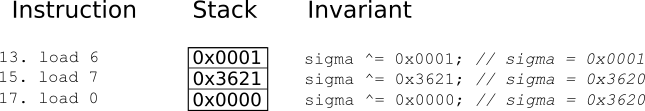
\includegraphics[scale=0.5]{figures/stackinvariantModified1.png}
\end{figure}
\begin{center}
%$\sigma = 0x3620, \sum\mathcal{S}_\mathcal{T} = 0x3620$ \ding{51}

$\sigma \oplus  \sum\mathcal{S}_\mathcal{T} = 0x3620 \oplus 0x3620 = 0x0000$ \ding{51}
\end{center}
Bit flip occured
\begin{figure}
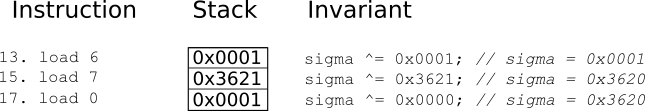
\includegraphics[scale=0.5]{figures/stackinvariantModified.png}\\~\\
\end{figure}
\begin{center}
%$\sigma = 0x3620, \sum\mathcal{S}_\mathcal{T} = 0x3621$ \ding{55}
$\sigma \oplus  \sum\mathcal{S}_\mathcal{T} = 0x3620 \oplus 0x3621 = 0x0001$ \ding{55}
\end{center}
\end{frame}